% !TEX encoding = UTF-8 Unicode

\documentclass[twocolumn,10pt,a4j]{ltjsarticle}
\usepackage{kougai}

\title{ゲームに最適化されたベンチマークソフトの開発}
\author{2032087 大司 陽輝  指導教員 須田 宇宙 准教授}
\date{}

\begin{document}

\maketitle

\section{はじめに}
%背景
ゲームに注目が集まりゲームが快適に行えるパソコン(ゲーミングパソコン)の需要が増加している.


%問題点
しかし,ゲームが快適に行えるパソコンを選ぶには専門の知識が必要となる.
それに対して,ベンチマークソフトを使うことで,ゲームに対してパソコンがスムーズに動作するかの快適度を知る事ができる.
ここでいう快適度は、アイテムなどの境目が鮮明に判断でき、文字の粗や色ずれが起きない程度とし、操作に遅延を感じないことを指標とする。
しかし、ゲームによってPCへの負荷が異なるため、既存のベンチマークソフトでは、様々なジャンルのゲームに対応したベンチマークソフトがない。

%目的
従って本研究ではテクスチャや,敵の数などのパラメーターを調整できる,汎用性のあるベンチマークソフトの開発を目的とする.

\section{ゲームがどう動いているか}
ゲームにはCPU、GPU、メモリの三つのパーツが主に重要となる。
CPUでは、ゲームの敵のキャラクターの行動を決めるAIや、サウンドなどを処理している。
GPUでは、ゲームの演出を処理し、マップやキャラクターのレンダリングや、テクスチャのマッピング、シェーディングの処理が行われている。
メモリは、キャラクターのデータや、画像、サウンドなどのデータを一時的に記憶するために使用されている。

%2章
ベンチマークソフトに実装する機能を検討する際、ゲームの処理に時間のかかる要素を知るために、FINAL FANTASY XV WINDOWS EDITIONの各グラフィックパラメーターを変化させた結果、グラフィックアセット、テクスチャフィルタリング、高解像度の処理に時間のかかることが明らかになった。
グラフィックアセットを模倣することは難しいため、テクスチャフィルタリングを調整できる機能を追加する。
また、近年では光線などを追跡することで、ある点において観測される像などをシミュレートすることでより再現性の高い表現のできるレイトレーシングにも注目されており、処理に時間のかかる要素であるため、レイトレーシングにも対応できる機能を実装する。
さらに、ベンチマークを結果からどのパーツで性能を最大限に引き出せていないかや、どのパーツを変更することでPCの性能を効果的に向上させられるかを判断できる機能を追加する。
さらに、ベンチマークは各パラメーターを変更して、何度も繰り返す作業が伴うため、自動でパラメーターを変更しつつ、ループする機能も加える。




\begin{figure}[h]
\begin{center}
 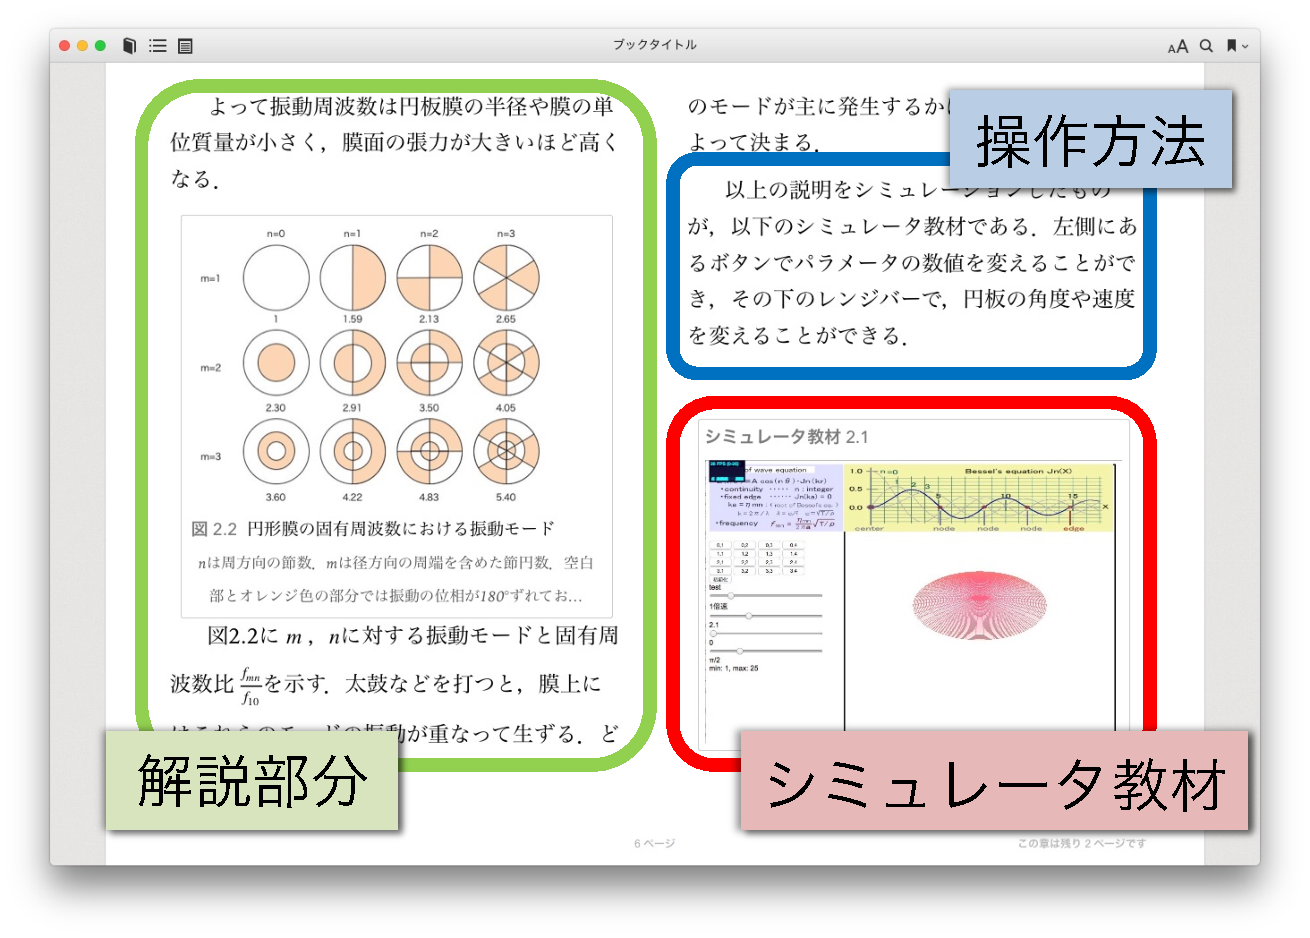
\includegraphics[clip,width=85mm,height=55mm]{textbook.pdf}
\end{center}
 \caption{電子教科書サンプル}
 \label{fig:教科書}
\end{figure}

\section{やること・やったこと}

3章には,中間審査用の梗概では実際に行う作業について(図を用いて)説明する.
最終審査用の梗概では,やったことを示す.
コンテンツを作成した場合にはコンテンツのスクリーンショットなどを用いる.
調査が主であれば,調査の概要と結果のグラフなどを使用する.

この文章では1章が長すぎるので,見た目のバランスが悪い.
通常の梗概の割合は左側に1章と2章,右側に3章と4章のように並ぶ.
もちろん多少の前後は有るので,きっちりと合わせなくても良い.

通常,図は2枚程度である.
図1枚+表1面でも構わない.
梗概を書き始める前に,使用する図を決めてからレイアウトしていくと雰囲気がつかみやすくて良い.




\section{今後の予定}
中間審査用の梗概では4章のタイトルとして「今後の予定」,最終審査用の梗概では「おわりに」などを用いる.
たいてい2〜3行程度でまとめる.

\begin{thebibliography}{99}
\bibitem{suda2018} 須田宇宙: ``音響科学e-Learning教材'', \url{https://www.sudalab.net/}, 2018/7/19参照
\end{thebibliography}

\end{document}
